\documentclass[11pt]{beamer}
\usetheme{CambridgeUS}
\usepackage[utf8]{inputenc}
\usepackage{amsmath}
\usepackage{amsfonts}
\usepackage{amssymb}
\usepackage{graphicx}
\usepackage{pgfpages}
\usepackage{framed}
\usepackage{xcolor}
\usepackage[most]{tcolorbox}
\usepackage{soul}
\usepackage{empheq}

\newcommand*{\itemimg}[1]{%
  \raisebox{-.3\baselineskip}{%
    \includegraphics[
      height=\baselineskip,
      width=\baselineskip,
      keepaspectratio,
    ]{#1}%
  }%
}

\newtcbox{\mymath}[1][]{%
    nobeforeafter, math upper, tcbox raise base,
    enhanced, colframe=blue!30!black,
    colback=blue!10, boxrule=1pt,
    #1}

\newcommand{\highlight}[1]{%
  \colorbox{yellow!100}{$\displaystyle#1$}}

\author{Giovanni Della Lunga\\{\footnotesize giovanni.dellalunga@unibo.it}}
%\title{1 - Introduction to Machine Learning}
%\title{2.1 - Data Pre-Processing}
\title{4.1 - Model Valuation and Selection}
%\title{4.2 - Decision Trees}
%\title{6 - Text Vectorization}
%\title{7 - Classification for Text Analysis}
%\title{8 - Clustering for Text Similarity}
%\title{9 - Information Extraction}
\subtitle{} % (optional)
\setbeamercovered{transparent} 
%\institute{Introduction to Machine Learning for Finance} 
\date{Bologna - February-April, 2025} 

\begin{document}

\begin{frame}
\titlepage
\end{frame}

\AtBeginSection[]
{
%	\begin{frame}<beamer>
%  		\frametitle{Outline}
%  		\tableofcontents[currentsection]
%	\end{frame}
  	\begin{frame}
  		\vfill
  		\centering
  		\begin{beamercolorbox}	[sep=8pt,center,shadow=true,rounded=true]{title}  		\usebeamerfont{title}\insertsectionhead\par%
  		\end{beamercolorbox}
  		\vfill
  \end{frame}
}
\AtBeginSubsection{\frame{\subsectionpage}}


%______________________________________________________________________________
%
\section{Accuracy Metrics}
%______________________________________________________________________________
%
\begin{frame}{Accuracy Metrics: how to choose a Model?}
	\begin{itemize}
		\item Let's consider a simple problem of bynary classsification. Example: you have to classify bank custumer into good or bad wrt the credit whortiness;
		\item Probably the first thing you think is to measure the godness of your model using the classification accuracy...
		\item ... but this would turn out to be a very bad idea

	\end{itemize}
	\vspace{1.5cm}
	Why?
\end{frame}
%..................................................................
\begin{frame}{Accuracy Metrics: how to choose a Model?}
Credit Classification Example
\begin{itemize}
		\item Train logistic regression model (say y=1 if the client is bad and 0 otherwise);
\item Find that you got 10\% error on test set (90\% correct classification);
\item Only 8\% of clients are bad clients. You have a very \textbf{unbalanced} or skewed sample;
\end{itemize}
\vspace{0.5cm}
\textbf{function predictBadLoad(x)\\}
\textbf{\hspace{1cm} return 0\\}
\vspace{0.5cm}
This very stupid model has a classification accuracy of 92\%!!!

\end{frame}
%..................................................................
\begin{frame}{Threshold}
	\begin{itemize}
		\item The threshold is an arbitrarily decided upon point between 0.0 and 1.0 that serves as your "cutoff" for which predicted probabilities you want to consider a True or a False, a Yes or a No, a 1 or a 0. 
		\item Who decides it? 
		\item You do, or whomever the decision-maker happens to be. 
		\item You may have assumed this threshold is naturally located right in the middle, at 0.5, but you can move that threshold.
	\end{itemize}
\end{frame}
%..................................................................
\begin{frame}{Threshold}
	\begin{itemize}
		\item Why would you want to do that? 
		\item Reasons include: 
		\item a) You are conservative about your guesses, so you set the threshold for a "Yes" to 0.7 (or 70\%, if you will). Anything predicted to have less than a 70\% probability is just too risky for you. 
		\item b) Alternatively, a risk-taker may want to call anything over 0.35 probability a "Yes", so that they don`t miss any opportunities. 
		\item c) Lastly, perhaps you want to use the threshold that gives the highest performance, for whatever metric you choose. 
	\end{itemize}
\end{frame}
%..................................................................
\begin{frame}{Confusion Matrix}
\begin{columns}[T] % align columns
\begin{column}{.48\textwidth}
        \begin{itemize}
		\item A confusion matrix is $N*N$ dimension matrix wherein one axis represents \textbf{Actual} label while the other axis represents \textbf{Predicted} label.
		\item Confusion Matrix is the most intuitive and basic metric from which we can obtain various other metrics like precision, recall, accuracy, F1 score, AUC - ROC.
        \end{itemize}
\end{column}%
\hfill%
\begin{column}{.48\textwidth}
    %\fbox{
        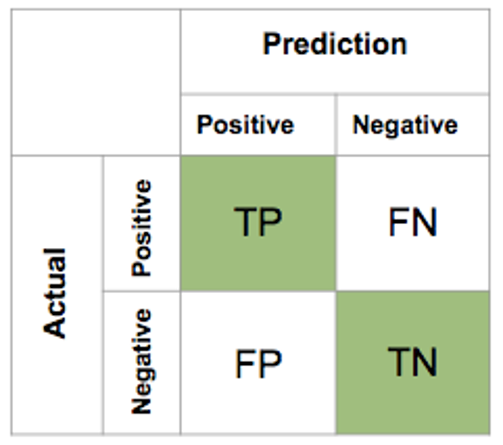
\includegraphics[width=\linewidth]{../05-pictures/lesson-4-1_pic_0.png}
    %}
\end{column}%
\end{columns}
\end{frame}
%..................................................................
\begin{frame}{Confusion Matrix}
	\begin{itemize}
		\item \footnotesize{For a better understanding of what TP, FP, TN, and FN are, we will consider an example of:  \textbf{If received mail is spam or ham.}
		\item \textbf{Positive} - Mail received is ham
		\item \textbf{Negative} - Mail received is spam 
		\item \textbf{$\Rightarrow$   True Positive (TP)}: It represents the predicted label is positive and also actual label is positive - correctly predicted. We predicted mail received is `ham` (positive) and actual mail received is also `ham` (positive).
		\item \textbf{$\Rightarrow$   True Negative (TN)}: It represents the predicted label is negative and also actual label is negative - correctly predicted. We predicted mail received is `spam` (negative) and actual mail received is also `spam` (negative).
		\item \textbf{$\Rightarrow$   False Negative (FN)}: It represents the predicted label is negative but the actual label is positive - wrongly predicted. We predicted mail received is `spam` (negative) but actual mail received is `ham` (positive).
		\item \textbf{$\Rightarrow$   False Positive (FP)}: It represents the predicted label is positive but the actual label is negative - wrongly predicted. We predicted mail received is `ham` (positive) but actual mail received is `spam` (negative).}
	\end{itemize}
\end{frame}
%..................................................................
\begin{frame}{Precision}
	\begin{itemize}
		\item \textbf{General Definition}: Precision measures what proportion of predicted positive label is actually positive.
		\item \textbf{Precision} can be expressed in terms of True Positive and False Positive: $$\text{Precision} = \frac{\text{True Positive}}{\text{True Positive}+\text{False Positive}}$$
		\item As `False Positive` decreases, our precision increases and vice-versa
		\item When to use Precision?
		\item Precision is used when we want to mostly focus on false-positive i.e to decrease false-positive value thereby increase precision value. 
		\item A question might arise why we want to mostly focus on false-positive and not false-negative. The answer to this question depends on the context.
	\end{itemize}
\end{frame}
%..................................................................
\begin{frame}{Recall/Sensitivity}
	\begin{itemize}
		\item \textbf{General Definition}: Recall measures what proportion of actual positive label is correctly predicted as positive.
		\item To explain recall and its use case, we shall consider `Cancer Diagnosis` example i.e we have to predict if a patient is diagnosed with cancer or not.
		\item \textbf{Positive} - Patient diagnosed with cancer.
		\item \textbf{Negative} - Patient not diagnosed with cancer.
		\item Recall in terms of True Positive and False Negative: $$\text{Recall} = \frac{\text{True Positive}}{\text{True Positive}+\text{False Negative}}$$
		\item From the above formula in the image, we can analyze that as `False Negative` decreases, our recall increases and vice-versa.
	\end{itemize}
\end{frame}
%..................................................................
\begin{frame}{Recall/Sensitivity}
	\begin{itemize}
		\item When to use Recall?
		\item Recall is used when we want to mostly focus on false-negative i.e to decrease false negative value thereby increase recall value. 
		\item A question might arise why we want to mostly focus on a false-negative and not false positive. 
		\item To answer this question, let us consider `Cancer Diagnosis` example...
	\end{itemize}
\end{frame}
%..................................................................
\begin{frame}{Recall/Sensitivity}
	\begin{itemize}
		\item \textbf{False Negative (FN)}
		\item It represents our predicted label is negative but the actual label is positive - wrongly predicted. 
		\item Applying false negative on our example- it means we have predicted that the patient is not diagnosed with cancer but the actual patient is diagnosed with cancer. 
		\item If this is the case, patient, as per prediction might not get treatment to cure cancer. 
		\item But the truth is patient is diagnosed with cancer. 
		\item Our wrong negative prediction will lead to death of a patient. 
		\item So, \textbf{we mostly focus on false-negative} value and try to decrease it to the least possible value.
	\end{itemize}
\end{frame}
%..................................................................
\begin{frame}{Recall/Sensitivity}
	\begin{itemize}
		\item \textbf{False Positive (FP)} 
		\item It represents our predicted label is positive but the actual label is negative - wrongly predicted. 
		\item Applying false positive on our example- it means we have predicted that the patient is diagnosed with cancer but the actual patient is not diagnosed with cancer. 
		\item If this is the case, patient, as per prediction will get check-up for cancer diagnosis. 
		\item To his happiness, he will come to know that he is not diagnosed with cancer. Hurrah! He is free from cancer now. 
		\item So, we don`t much focus on false-positive value.
	\end{itemize}
\end{frame}
%..................................................................
\begin{frame}{F1-Score}
	\begin{itemize}
		\item F1-score is another one of the good performance metrics which leverages both precision and recall metrics. 
		\item F1-score can be obtained by simply taking `Harmonic Mean` of precision and recall. 
		\item Unlike precision which mostly focuses on false-positive and recall which mostly focuses on false-negative, \textbf{F1-score focuses on both false positive and false negative}.
	\end{itemize}
\end{frame}
%..................................................................
\begin{frame}{F1-Score}
	\begin{itemize}
		\item F1-score in terms of Precision and Recall;
		\item The F-Score is the Harmonic Mean of Precision and Recall:$$F = \frac{2}{ \frac{1}{\text{Recall}} + \frac{1}{\text{Precision}}}$$
		\item  Alternatively:$$F = 2\times \frac{\text{Precision}\times \text{Recall}}{\text{Precision}+\text{Recall}}$$
		\item When to use F1-score:
		\item As mentioned above, F1-score focuses on both false positive and false negative and try to decrease both false positive and false negative thereby increase F1-score.
	\end{itemize}
\end{frame}
%..................................................................
\begin{frame}{AUC - ROC curve}
	\begin{itemize}
		\item AUC - ROC is one of the most important performance metric used to check model performance. 
		\item AUC - ROC is used for binary and also multi-class classification but mostly used in binary classification problems. 
		\item In this lesson, we will consider a binary class classification.
		\item AUC-ROC is a graphical representation of model performance. ROC is a probability curve and AUC is the measure of separability. 
		\item Depending on the threshold set, we can analyze how well our model has performed in separating two classes. 
		\item Higher the AUC better is our model in separating two classes.
	\end{itemize}
\end{frame}
%..................................................................
\begin{frame}{AUC - ROC curve}
\begin{columns}[T] % align columns
\begin{column}{.48\textwidth}
        \begin{itemize}
		\item Graphical representation of AUC - ROC
		\item Referring the image, we can see that AUC - ROC curve is plotted with FPR against TPR where FPR (False Positive Rate) is on X-axis while TPR (True Positive Rate) is on Y-axis. 
		\item The green curve represents ROC curve while the area/region under ROC curve (green curve) represents AUC.
        \end{itemize}
\end{column}%
\hfill%
\begin{column}{.48\textwidth}
    %\fbox{
        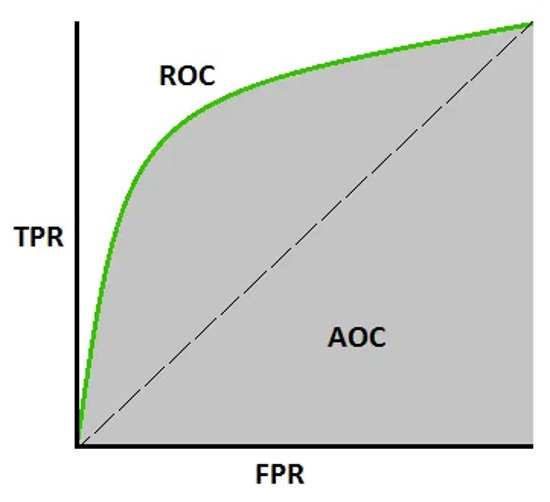
\includegraphics[width=\linewidth]{../05-pictures/lesson-4-1_pic_1.png}
    %}
\end{column}%
\end{columns}
\end{frame}
%..................................................................
\begin{frame}{AUC - ROC curve}
\begin{columns}[T] % align columns
\begin{column}{.48\textwidth}
        \begin{itemize}
		\item \textbf{True Positive Rate (TPR)}: TPR is nothing but Recall / Sensitivity. 
		\item The formula for TPR as follows: $$TPR=\frac{TP}{TP+FN}$$
        \end{itemize}
\end{column}%
\hfill%
\begin{column}{.48\textwidth}
    %\fbox{
        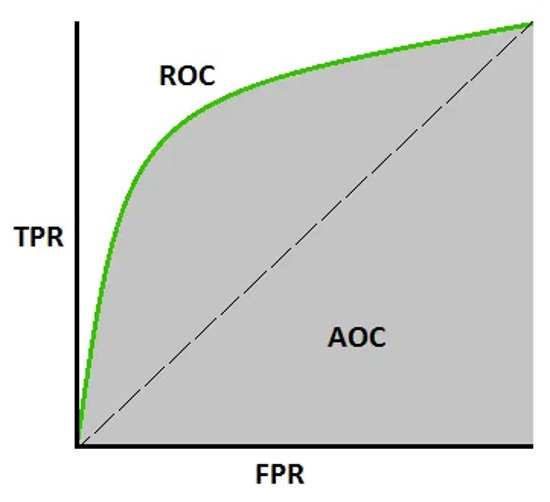
\includegraphics[width=\linewidth]{../05-pictures/lesson-4-1_pic_2.png}
    %}
\end{column}%
\end{columns}
\end{frame}
%..................................................................
\begin{frame}{AUC - ROC curve}
\begin{columns}[T] % align columns
\begin{column}{.48\textwidth}
        \begin{itemize}
		\item \textbf{False Positive Rate (FPR)}
		\item The formula for TPR as follows: $$FPR=\frac{FP}{TN+FP}$$
        \end{itemize}
\end{column}%
\hfill%
\begin{column}{.48\textwidth}
    %\fbox{
        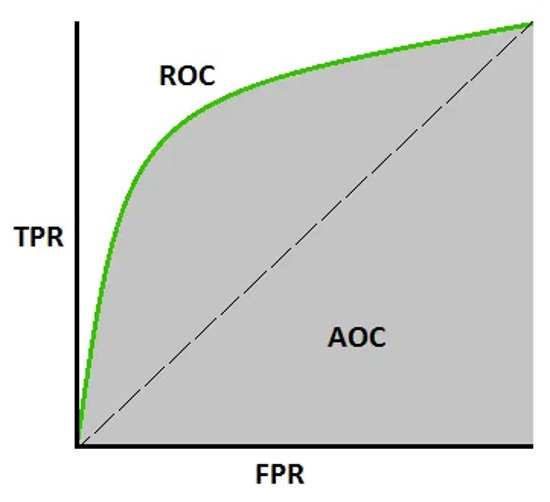
\includegraphics[width=\linewidth]{../05-pictures/lesson-4-1_pic_3.png}
    %}
\end{column}%
\end{columns}
\end{frame}
\begin{frame}{AUC - ROC curve}
	\begin{itemize}
		\item Interpretation of AUC-ROC curve
		\item Let`s now look into the analysis of binary class classification based on the AUC score and ROC curve...
	\end{itemize}
\end{frame}
%..................................................................
\begin{frame}{AUC - ROC curve}
	Threshold set to 0.5. There is no overlap between the two curves (green and red). This is the best model with AUC score of 1.0. This indicates that the probability of a model to separate positive and negative class is 1.0. In other words, we can say that there is 100\% chance model can separate positive and negative class.
	\begin{center}
	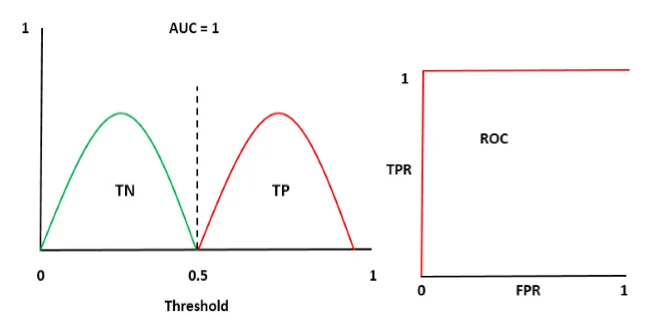
\includegraphics[scale=0.5]{../05-pictures/lesson-4-1_pic_4.png}
	\end{center}
\end{frame}
%..................................................................
\begin{frame}{AUC - ROC curve}
	Threshold set to 0.5. There is a little bit of overlap between the two curves (green and red). This is a good model with AUC score of 0.8. This indicates that the probability of a model to separate positive and negative class is 0.8. In other words, we can say that there is 80\% chance model can separate positive and negative class.
	\begin{center}
	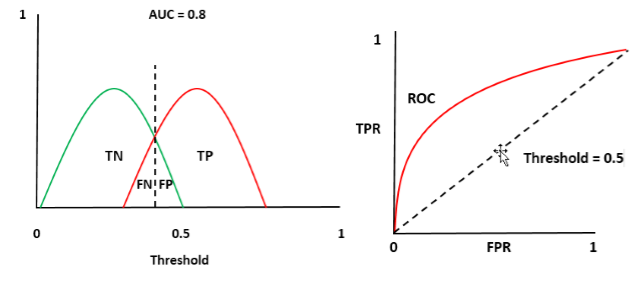
\includegraphics[scale=0.5]{../05-pictures/lesson-4-1_pic_5.png}
	\end{center}
\end{frame}
%..................................................................
\begin{frame}{AUC - ROC curve}
	Threshold set to 0.5. We can see the full overlap between the two curves (green and red). This is a bad model with AUC score of 0.5. This indicates that the probability of a model to separate positive and negative class is 0.5. In other words, we can say that there is 50\% chance model can separate positive and negative class.
	\begin{center}
	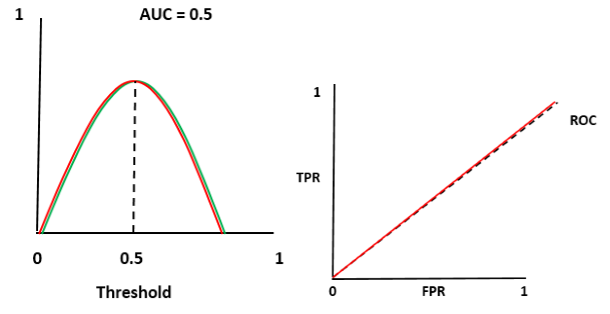
\includegraphics[scale=0.5]{../05-pictures/lesson-4-1_pic_6.png}
	\end{center}
\end{frame}
%..................................................................
\begin{frame}{Summary}
	\begin{itemize}
		\item \footnotesize{\textbf{Precision}: Precision measures what proportion of predicted positive label is actually positive. We mostly focus on false-positive value and try to decrease it to the least possible value thereby increase in precision value.
		\item \textbf{Recall}: Recall measures what proportion of actual positive label is correctly predicted as positive. We mostly focus on false-negative value and try to decrease it to the least possible value thereby increase in recall value.
		\item \textbf{F1-Score}: F1 Score is the `Harmonic Mean` of precision and recall. We focus on both false-positive and false-negative and try to decrease both false-positive and false-negative thereby increase F1 Score.
		\item \textbf{AUC- ROC curve}: It is a graphical representation of ROC curve and region/area under curve i.e AUC. It is mostly used in binary class classification. It interprets the probability or percentage of separability of positive and negative classes. Higher the AUC - ROC, better is our model in separating positive and negative classes.}
	\end{itemize}
\end{frame}
%______________________________________________________________________________
%
%\section{Model Selection}


%______________________________________________________________________________
%
\section{References and Credits}
%===================================================================================================
\begin{frame}{Bibliography}
\begin{thebibliography}{9}

\setbeamertemplate{bibliography item}[book]

\bibitem{1} John C. Hull, \textit{Machine Learning in Business: An Introduction to the World of Data Science}, Amazon, 2019.

\bibitem{2} Paul Wilmott, \textit{Machine Learning: An Applied Mathematics Introduction}, Panda Ohana Publishing, 2019.

\end{thebibliography}
\end{frame}
%===================================================================================================
\end{document}

%..................................................................
\begin{frame}{Notebook Reference}
\begin{columns}[T] % align columns
\begin{column}{.48\textwidth}
        \begin{itemize}
		\item \textbf{chapter-1-4} Notebook 
		\item[] In this notebook you will find an example of applying the metrics discussed in this section applied to a simple case of credit risk. Knowledge of logistic regression and credit risk issues is assumed.
        \end{itemize}
\end{column}%
\hfill%
\begin{column}{.48\textwidth}
    %\fbox{
        \includegraphics[width=\linewidth]{../05-pictures/letscode.png}
    %}
\end{column}%
\end{columns}
\end{frame}
%..................................................................
\begin{frame}{}
\begin{itemize}
\item 
\end{itemize}
\end{frame}
%..................................................................
\begin{frame}{}
\begin{itemize}
\item 
\end{itemize}
\end{frame}
%..................................................................
\begin{frame}{}
\begin{itemize}
\item 
\end{itemize}
\end{frame}
%..................................................................
\begin{frame}{}
\begin{itemize}
\item 
\end{itemize}
\end{frame}
